\vspace{-8pt}
\section{Introduction}%
\label{sec:intro}

\begin{figure}
\centering
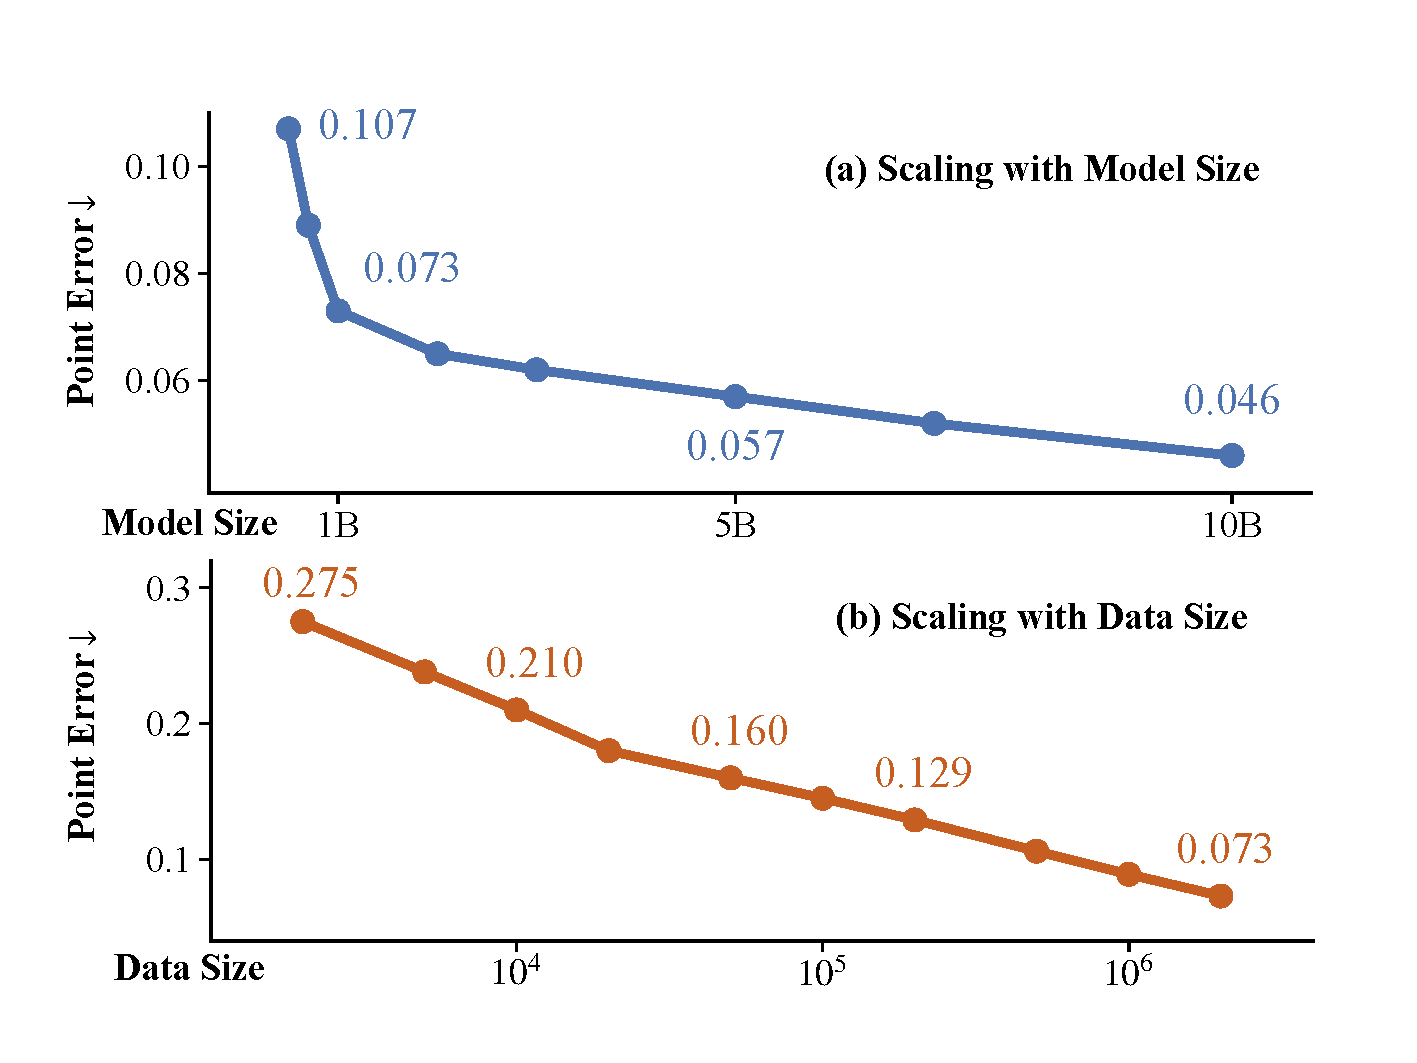
\includegraphics[width=0.95\linewidth]{figures/scale_v5_vector.pdf}
\caption{\textbf{Performance Gains from Data and Model Parameter Scaling.}
As model size increases from 0.2B to 10B parameters and data scale grows from 2K to 2M sequences, performance improves consistently, as measured by 3D point error (lower is better; note the different axis scales).
All models are trained on approximately the same number of tokens and evaluated by averaging over six datasets, with details provided in \cref{sec:benchmarking}.
}%
\label{fig:scale}
\vspace{-10pt}
\end{figure}




Recent work~\cite{wang24dust3r:, leroy24grounding, wang25vggt, wang25p3, lin25depth} has shown that feed-forward reconstruction models can, in many cases, match and even surpass traditional structure-from-motion (SfM) pipelines~\cite{hartley00multiple,snavely06photo,schonberger16structure-from-motion}.
Furthermore, the tokens learned by such models have been used as effective geometry-aware representations in many other tasks~\cite{li25spatial, abouzeid25geoaware-vla:, zeng25janusvln:,qian26xembodied:, zhang26spatialstack:, zhang26make, zheng25learning,bonnen26human-level,wang26let-geometry, huang26gen3r:, jang26repurposing, yang26cambrian-s:, szymanowicz26lagernvs,cao26vggt-det:, gao26vggt-segmentor:, zhao25spacemind:, yang25dense, vuong25improving, rao26augvla-3d:, zhou26generalizing, xu26vggt-mpr:, wu26mvggt:, lee253d-aware}.
This indicates that reconstruction can serve as a proxy task for learning representations useful for spatial understanding in general, with a foundational value.
However, compared to foundation models where the role of scale is well understood~\cite{simeoni25dinov3, kaplan20scaling, zhai22scaling}, this is less explored in 3D computer vision.
In this paper, we therefore ask whether feed-forward reconstruction models can be scaled up, and what benefits such scaling brings.
To answer this question, we introduce \method, scaling feed-forward reconstruction to significantly larger data and, optionally, model size than prior work.

Compared to VGGT~\cite{wang25vggt}, the new model introduces a number of architectural improvements, beginning with how it uses registers.
Recent works~\cite{darcet24vision, jiang25vision, marouani26revisiting} noted that vision transformers (ViTs) spontaneously use a small number of image tokens to carry global information, and introduced learnable registers to do so more directly and efficiently.
While VGGT already has per-frame registers, \method further introduces \emph{register attention}: in a subset of the global attention layers, information exchange among frames is restricted to the registers.
The updated registers then interact with other tokens locally within frame attention layers, thereby forming a bottleneck for aggregating and redistributing multi-frame information.
This design encourages the registers to aggregate information about the scene as a whole, and we also call them `scene' tokens.

There are two benefits to this design.
First, while in other architectures registers are often treated as auxiliary and discarded at inference time~\cite{darcet24vision}, we instead show that they carry useful global information.
In particular, although without explicit supervision, they provide useful features for vision-language-action (VLA) models and language alignment.
Second, register attention also improves efficiency.
Global attention is the main computational bottleneck in VGGT, but its attention maps are very sparse~\cite{shen26fastvggt:, wang25faster}.
We find that register attention, by aggregating global information, can also serve as an efficient substitute for full global attention.
Specifically, replacing 25\% of global attention layers with register attention incurs no measurable performance drop, while saving around 23\% FLOPs and 16\% memory in the backbone during training\footnote{Replacing \textit{all} global attention layers with register attention reduces FLOPs to just 6\% of the original, but leads to a considerable performance drop.}.

Registers aside, we also note that high-resolution convolutional layers in dense prediction heads (\eg, DPT) consume a disproportionate amount of GPU memory for storing forward activations, despite accounting for only a small fraction of the model's parameters.
Techniques like FSDP or gradient checkpointing cannot eliminate the cost of storing these activations.
Instead, our second change is to replace the most memory-intensive convolutional layers in the dense predictors with a single MLP followed by a pixel shuffle operator.
This uses little memory without performance degradation, both quantitatively and qualitatively.

Finally, in VGGT, we showed that multi-task training, where depth maps, point maps, and tracking features are supervised directly, is beneficial.
Here, we find that additional dense \textit{heads} are unnecessary to achieve these benefits.
Our third change is to still use multi-task \textit{losses}, but to retain only a single dense head for depth prediction and a single sparse head for camera prediction.

These three changes save 70\% of GPU memory during training and modestly improve inference speed.

In addition to efficiency, we find that the amount, diversity, and quality of the training data are critical for scaling.
In particular, handling \emph{dynamic} content is essential as it unlocks orders of magnitude more Internet-like videos for training.
Therefore, we develop a high-quality data annotation pipeline that can produce annotations for both rigid and dynamic videos at scale.
The pipeline integrates VLM-based pre-filtering, VGGT, COLMAP, modern image-matching models, and supervised geometric post-filtering.
Applied to around $40$ million internal Internet-style videos, the filtering pipeline retains $0.8$ million sequences with accurate annotations, roughly one-third of which contain dynamic content.
Combined with existing datasets (both real and synthetic), this yields a total of $4$M diverse scenes/sequences with accurate reconstruction annotations, more than $15\times$ as many as VGGT\@.

To further improve generalization, we introduce a self-supervised learning protocol inspired by DINO and related momentum teacher-student methods~\cite{caron21emerging, oquab24dinov2:,simeoni25dinov3, tarvainen17mean, he20momentum}.
We maintain teacher and student models initialized from a supervised \method checkpoint.
Both models process the same input sequences under different augmentations and frame permutations.
The student is trained to match the teacher's predictions and feature distribution (after aligning the frame order), while the teacher is updated via an exponential moving average of the student.
We use this protocol to train on $18$ million unlabeled videos.

These improvements allow us to investigate the scaling properties of feed-forward reconstruction models.
As illustrated in \cref{fig:scale}, we observe a consistent power-law-like improvement in reconstruction accuracy (measured by point error) as we increase the model capacity from 0.2B to 10B parameters and expand the training data from a few thousand to two million different sequences.

Overall, \method delivers a new level of feed-forward reconstruction performance, achieving state-of-the-art results in three static and three dynamic benchmarks by a wide margin.
In particular, it substantially outperforms post-optimization methods such as MegaSaM and recent feed-forward methods such as Depth Anything 3~\cite{lin25depth}.
On Sintel, \method attains AUC@$3^\circ$ of $40.0$ vs.\ $22.5$ (by $77\%$) and AUC@$30^\circ$ of $79.1$ vs.\ $58.3$ (by $35\%$) for camera estimation, as well as $\delta_{1.25}$ of $93.5$ vs.\ $74.1$ (by $26\%$) for depth estimation, while being $50\times$ faster than MegaSaM\@.
Finally, we show that the learned registers can be reused beyond reconstruction, improving VLA models and supporting alignment with language.

\begin{figure*}
\centering
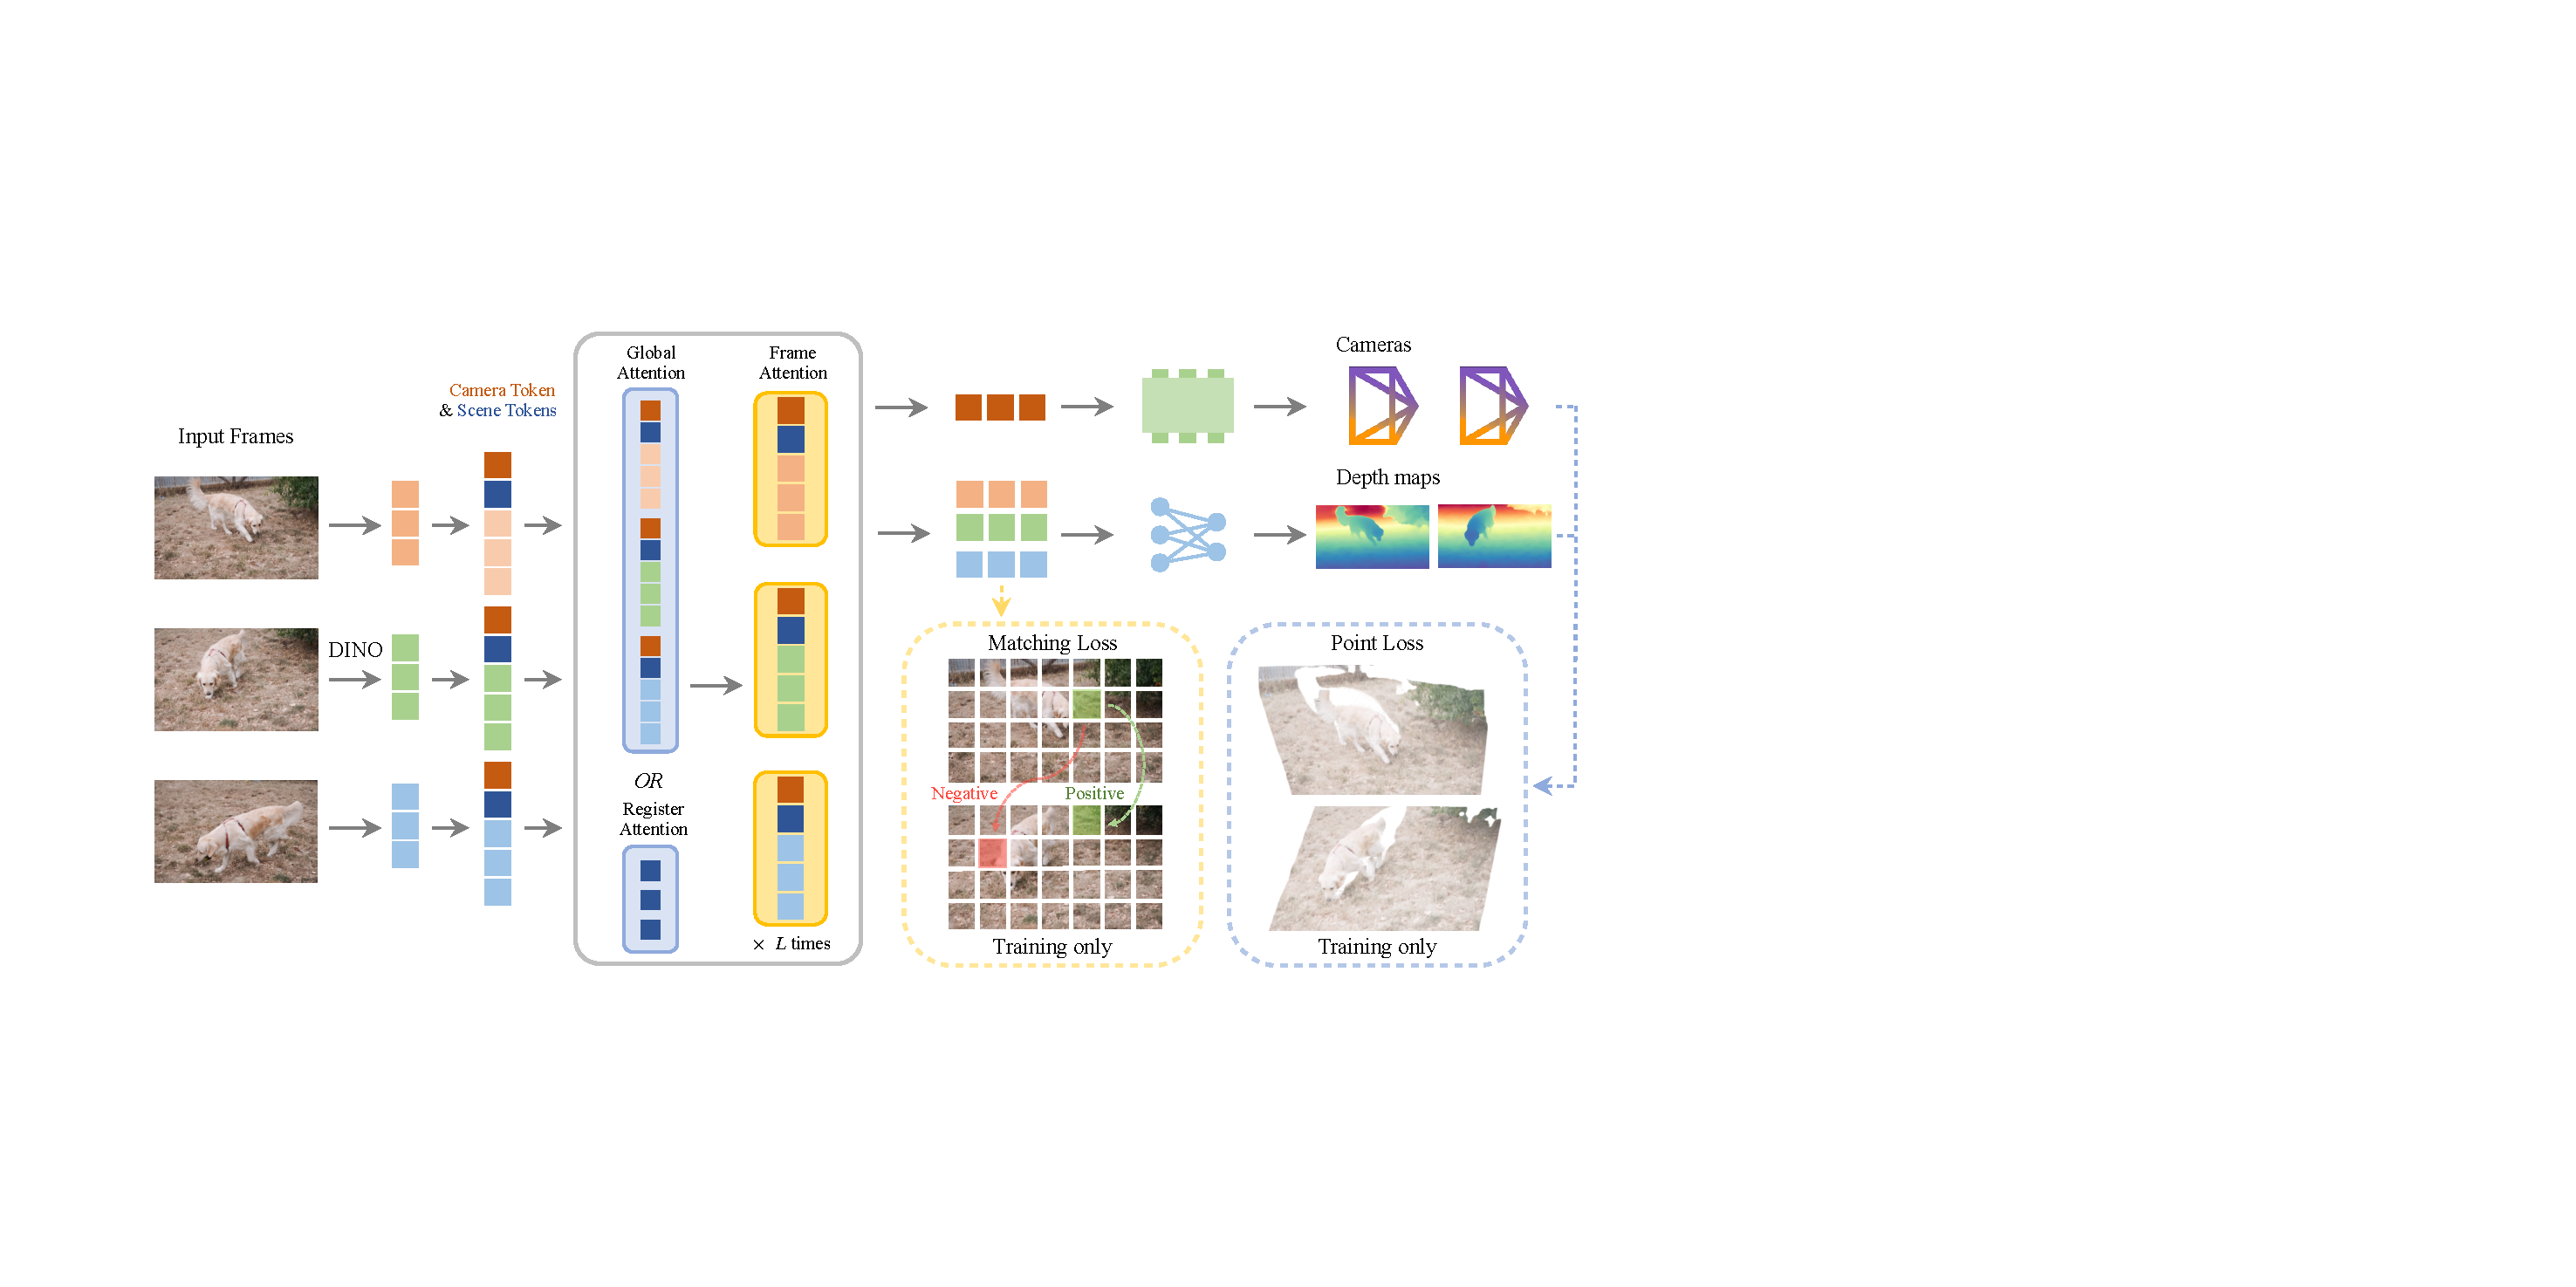
\includegraphics[width=0.95\textwidth]{figures/architecture_v8.pdf}
\vspace{-2pt}
\caption{\textbf{Architecture Overview.} \method appends camera and scene tokens (registers) to image tokens, and then alternates between global attention (or register attention) and frame attention layers.
We replace the redundant dense heads of VGGT with training-only losses.
}%
\label{fig:architecture}
\vspace{-10pt}
\end{figure*}





